\begin{vbframe}{Linear SVM -- Functionality}

\maketag{SUPERVISED} \maketag{CLASSIFICATION} \maketag{PARAMETRIC} 
\maketag{BLACK-BOX} 
\medskip

\highlight{General idea}

\begin{itemize}
  \item Find linear decision boundary (\textbf{separating hyperplane}) that 
  best separates classes
  \begin{itemize}
    \item \textbf{Hard-margin} SVM: maximize distance (\textbf{margin} 
    $\gamma$ > 0) to closest members (\textbf{support vectors, SV}) on each 
    side of decision boundary
    \item \textbf{Soft-margin} SVM: relax separation to allowing margin 
    violations $\rightarrow$ maximize margin while minimizing violations
  \end{itemize}
  \item 3 types of training points
  \begin{itemize}
    \item \textbf{non-SVs} with no impact on decision boundary
    \item \textbf{SVs} located exactly on decision boundary
    \item \textbf{margin violators}
  \end{itemize}
\end{itemize}

\medskip

\highlight{Hypothesis space} ~~
$\Hspace = \left\{f: \Xspace \to \R ~|~\fx = \thetab^\top \xv + \theta_0
\right\}$
 ~~ \textcolor{blue}{separater intercept notwendig?}

\framebreak

\medskip
\footnotesize
\begin{minipage}{0.6\textwidth}
  \centering
  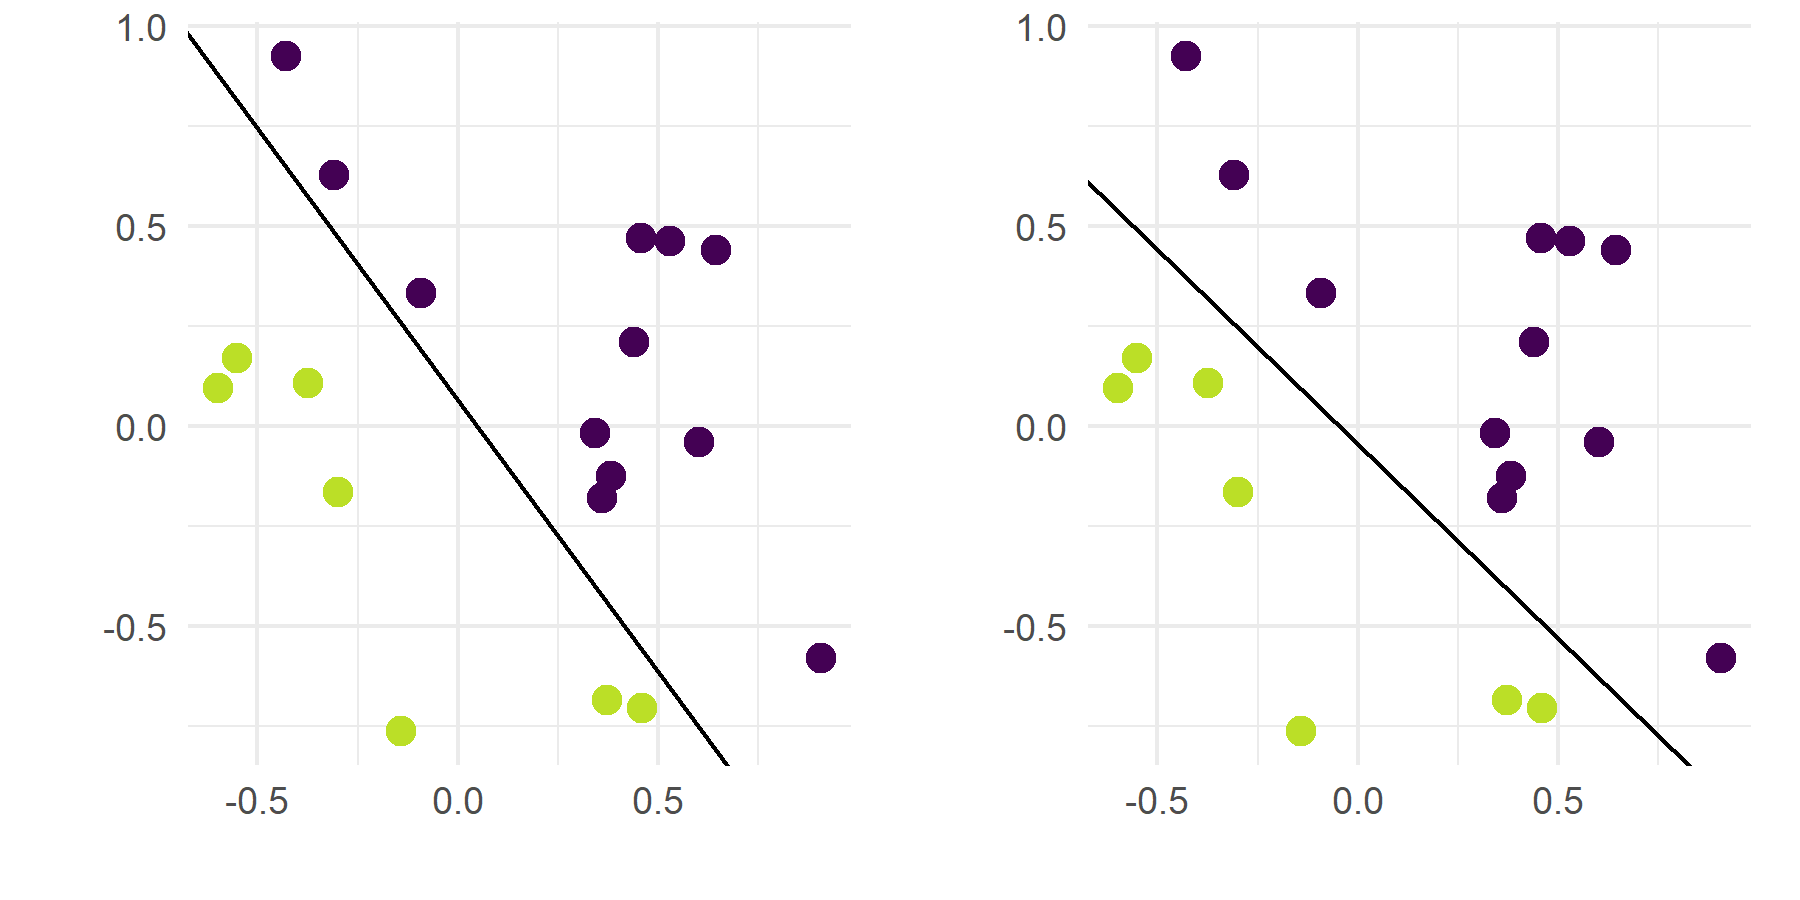
\includegraphics[width=0.9\textwidth]{
  ../slides/linear-svm/figure/linear_classif_1.png}  \\
  \tiny{Hard-margin SVM: margin is maximized by boundary on the right}
\end{minipage}
\hfill
\begin{minipage}{0.3\textwidth}
  \centering
    %https://docs.google.com/presentation/d/1g7q1hbTNmQeuRWQIM8SF9l6iKWmJyuhyhm3s9QjA0jM/edit?usp=sharing
  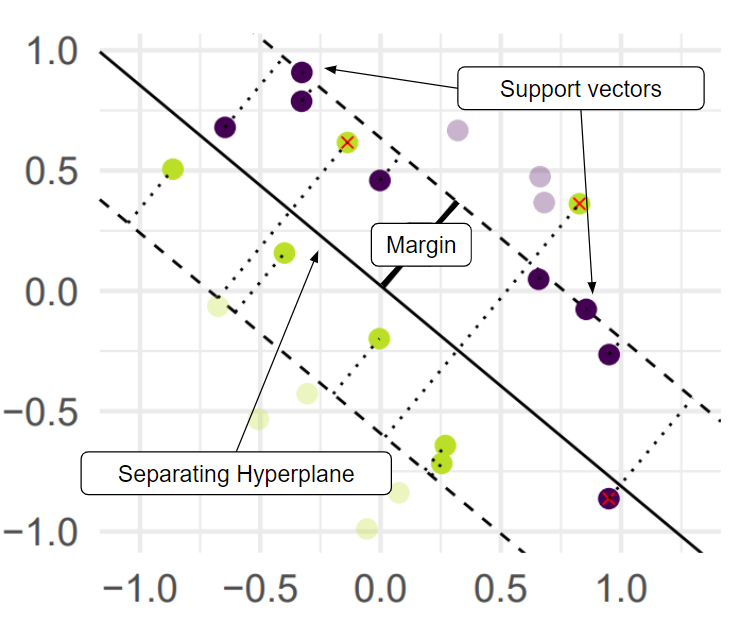
\includegraphics[width=1.1\textwidth]{figure/svm_wording.png} \\
  \tiny{Soft-margin SVM with margin violations}
\end{minipage}

\medskip

\highlight{Dual problem} ~~ %lecture_cim2\2020\08-linear-svm\slides-3-soft-margin-svm.Rnw
\begin{eqnarray*}
    & \max\limits_{\alphav \in \R^n} & \dualobj \\
    & \text{s.t. } & 0 \le \alpha_i \le C ~~ \forall i \in \nset ~~ (C = \infty
    \text{ for hard-margin SVM)}, \\
    & \quad & \sum_{i=1}^n \alpha_i \yi = 0
\end{eqnarray*}

\framebreak

\highlight{Empirical risk}

Soft-margin SVM also interpretable as \textbf{L2-regularized ERM}: 

\begin{minipage}[b]{0.58\textwidth}
  $$ \frac{1}{2} \|\thetab\|^2 + C \sumin \Lxyi$$ 
  with  
  \begin{itemize}
    \item $\|\thetab\| = 1 / \gamma$,\\
    \item $C > 0$: penalization for missclassified data points
    \item $\Lyf = \max(1-yf, 0)$: \textbf{hinge} loss \\
    $\rightarrow$ other loss functions applicable (e.g., \textbf{Huber} loss)
  \end{itemize}
\end{minipage}
\begin{minipage}[b]{0.4\textwidth}
  \centering
  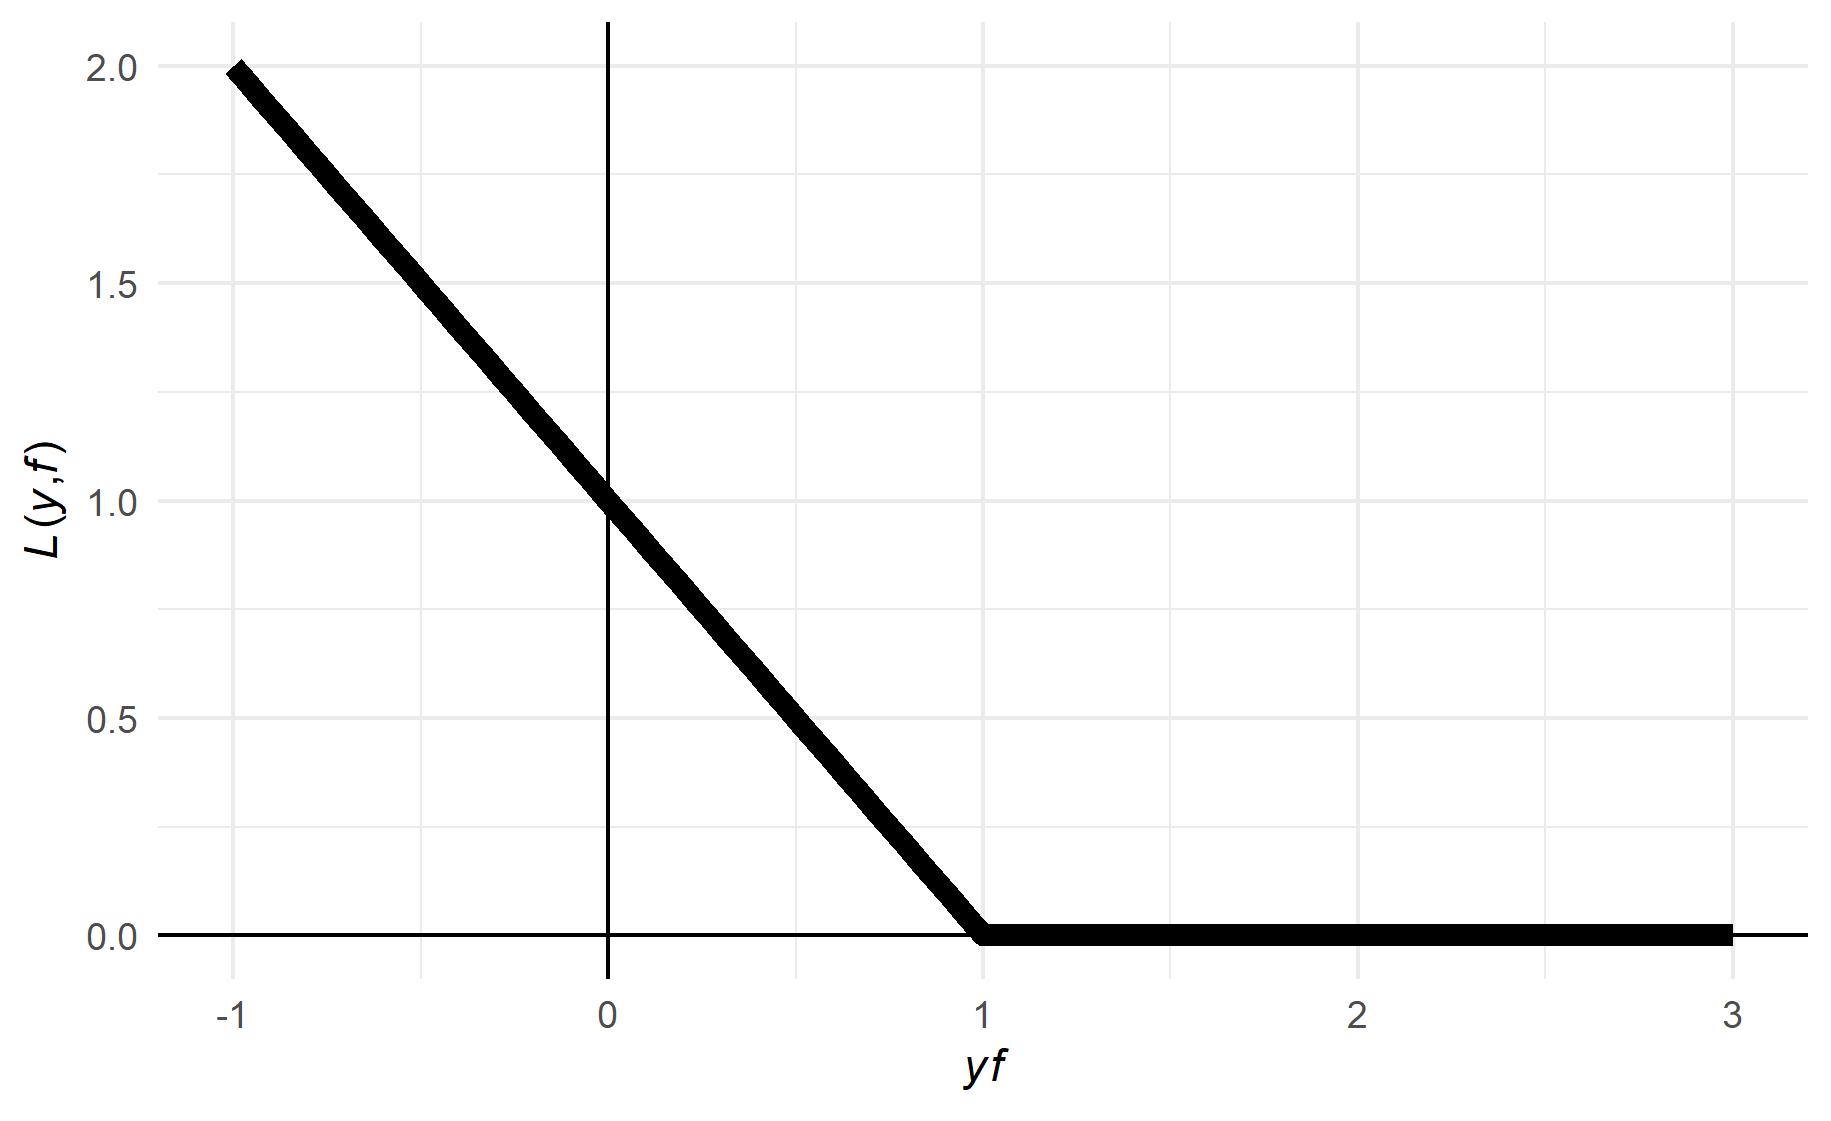
\includegraphics[height=0.4\textwidth, keepaspectratio=true]{
  figure/plot-hinge-loss.png}
\end{minipage}

\medskip

\highlight{Optimization}

\begin{itemize}
  \item Typically, tackling \textbf{dual} problem (though feasible 
  in corresponding primal) via \textbf{quadratic programming}
  \item Popular: \textbf{sequential minimal optimization} $\rightarrow$ 
  iterative algorithm based on breaking down objective into bivariate quadratic 
  problems with analytical solutions
\end{itemize}
\medskip

\highlight{Hyperparameters} ~~ Cost parameter \textbf{$C$}

\end{vbframe}

% ------------------------------------------------------------------------------

\setdraft

\begin{frame}{Linear SVM -- Pro's \& Con's}

\begin{columns}[onlytextwidth]
  \begin{column}{0.5\textwidth}
    \highlight{Advantages}
    \footnotesize
    \begin{itemize}
      % \positem High \textbf{accuracy}
      \positem Often \textbf{sparse} solution
      \positem Robust against overfitting (\textbf{regularized}); especially in 
      high-dimensional space
      \positem \textbf{Stable} solutions, as non-SV do not influence decision 
      boundary
      %\positem \textbf{memory efficient} (only use non-SVs)
    \end{itemize}
  \end{column}

  \begin{column}{0.5\textwidth}
    \highlight{Disadvantages}
    \footnotesize
    \begin{itemize}
      \negitem \textbf{Costly} implementation; long training times
      \negitem \textbf{Limited scalability} to larger data sets 
      \textcolor{blue}{\textbf{??}}
      \negitem Confined to \textbf{linear separation}
      \negitem Poor \textbf{interpretability}
    \end{itemize}
  \end{column}
\end{columns}

\vfill

\small

\conclbox{Very accurate solution for high-dimensional data that is linearly separable}

\end{frame}

\undraft

% ------------------------------------------------------------------------------

\begin{frame}{Linear SVM -- Practical hints}

\footnotesize

  \highlight{Preprocessing} \\
  Features must be rescaled before applying SVMs.
  
  \medskip
  
  \highlight{Tuning} \\
  Cost parameter $C$ must be tuned and has strong influence on resulting 
  separating hyperplane. 

  \medskip

  \highlight{Implementation} 
  \begin{itemize}
    \item \textbf{R:} \texttt{mlr3} learners \texttt{LearnerClassifSVM} / 
    \texttt{LearnerRegrSVM}, calling \texttt{svm()} from \texttt{libsvm}
    \item \textbf{Python:} \texttt{sklearn.svm.SVC} from package 
    \texttt{scikit-learn} / package \texttt{libSVM}
  \end{itemize}

\end{frame}
